\chapter{Introduction}

This chapter is dedicated to the general introduction of the problem at hand and previous work and research that is relevant for this project.

\section{Goal}

\gls{ml} and Neural Networks have shown to be extremely potent and versatile in solving vast variety of problems across different fields. One research field that has been popular and challenging in the last few years is \gls{co}. \gls{co} includes problems such as \gls{mis} and \gls{mwm}. Such problems can be viewed in the context of graphs. \gls{gnn} is a subclass of \gls{nn}s designed specifically for solving problems related to graphs, but there are some problems that have not yet been solved efficiently with \gls{gnn}s. The goal of this project is: "To find out whether a \gls{gnn} can outperform greedy algorithms at solving \gls{mwm}. 

\section{Background}
\label{sec:background}

Many researches have been done related to \gls{gnn}s in the past years. 

Lorenzo Brusca and Lars C. P. M. Quaedvlieg et al. \cite{brusca2023maximum} showed a self-training \gls{gnn} for \gls{mis}. 

Schuetz et. al. made an unsupervised \gls{gnn} \cite{Schuetz2022} for solving \gls{mis} and Angelini and Ricci-Tersenghi \cite{Angelini2022} compared  its performance to greedy algorithms and reported some problems with \gls{gnn}s performance.

The reason \gls{mis} solving is mentioned so much here is because the problems are to some degree related as algorithm probmels often are. There will be concrete examples in the Methodology and Data chapter. \gls{mis} is also more often a subject to research and researches on \gls{mwm} are not that common. Bohao Wu and Lingli Li tried to solve \gls{mwm} using deep reinforcement learning \cite{WU2022400} and reporting that "Experimental results show that L2M outperforms state-of-the-art algorithms."



\section{Project structure}

The rest of this document has the following structure:

\begin{enumerate}

\item Methodology and Data:

This Chapter will focus on how the research was done and also explain core concepts of gls{nn}s and the general procedure of training a gls{nn}. Then the specifics of this case will be discussed and main challenges mentioned. The progress made step by step and the reasoning behind changes and choices made along the way will be shown. The chapter will also analyze the data used for training the model and evaluating results along with justification for the chosen data. The temporary results are also included in this Chapter but not the final results.

\item Results:

This Chapter will focus on analyzing the final results and comparing them with the expactations.

\item Conclusion:

Here the conclusion for this project will be drawn regarding whether the results gave any meaningfull insight and what future work can be done for improvements.

\end{enumerate}


\subsection{Listings}
You can do listings, like in Listing~\ref{ListingReference}
\begin{lstlisting}[caption={[Short caption]Look at this cool listing. Find the rest in Appendix~\ref{Listing}},label=ListingReference]
$ java -jar myAwesomeCode.jar
\end{lstlisting}

You can also do language highlighting for instance with Golang:
And in line~\ref{LineThatDoesSomething} of Listing~\ref{ListingGolang} you can see that we can ref to lines in listings.

\begin{lstlisting}[caption={Hello world in Golang},label=ListingGolang,escapechar=|]
package main

import "fmt"

func main() {
    fmt.Println("hello world") |\label{LineThatDoesSomething}|
}

\end{lstlisting}

\subsection{Figures}

Example of a centred figure
\begin{figure}[H]
    \centering
    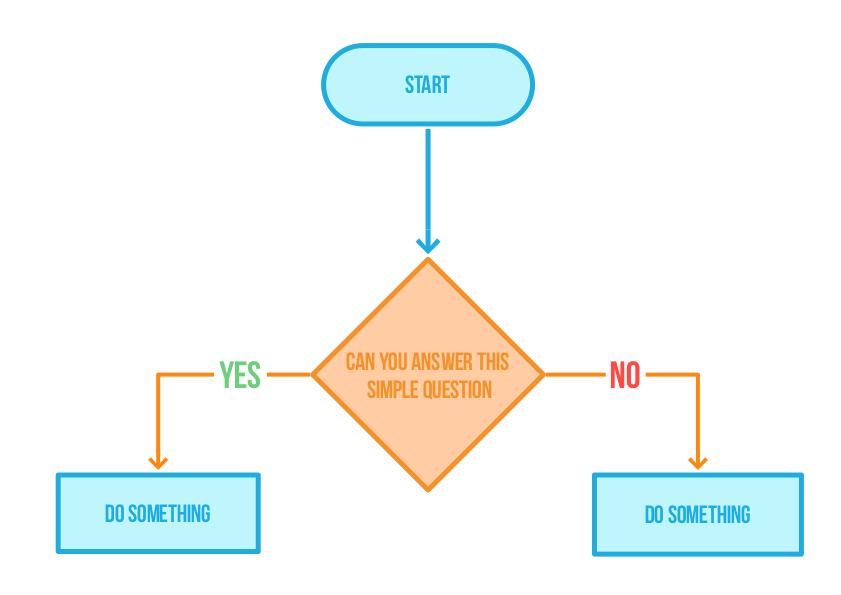
\includegraphics[scale=0.5]{figures/Flowchart}
    \caption{Caption for flowchart}
  	\medskip 
	\hspace*{15pt}\hbox{\scriptsize Credit: Acme company makes everything \url{https://acme.com/}}
    \label{FlowchartFigure}
\end{figure}

\subsection{Tables}

We can also do tables. Protip: use \url{https://www.tablesgenerator.com/} for generating tables.
\begin{table}[H]
\centering
\caption{Caption of table}
\label{TableLabel}
\begin{tabular}{|l|l|l|}
\hline
Title1 & Title2 & Title3 \\ \hline
data1  & data2  & data3  \\ \hline
\end{tabular}
\end{table}

\subsection{\gls{git}}

The whole project can be seen here: \url{https://github.com/nikitazaicev/Master}